\section{Optimal Flow on a Data Collection Network}

\textbf{(a)}
With the incidence convention in the problem, \((Af)_i\) is the flow entering node \(i\) minus the flow leaving node \(i\). Conservation gives
\[
(Af)_i+s_i=0
\]
for each regular node, so
\[
Af=-s
\]
The optimization problem is therefore
\[
\min_f \frac{1}{n}\|f\|_2^2
\qquad
\text{subject to}\qquad
Af=-s
\]
The factor \(1/n\) does not change the optimizer. Since the graph is connected to the destination node, the reduced incidence matrix \(A\) has linearly independent rows. Thus \(AA^T\) is invertible, and the minimum-norm feasible flow is
\[
f^\star=-A^T(AA^T)^{-1}s
\]

\textbf{(b)}
Using the arc directions in the figure,
\[
A=
\begin{bmatrix}
-1&1&-1&-1&0&0&0\\
0&-1&0&0&-1&0&0\\
0&0&0&1&1&-1&0\\
0&0&1&0&0&1&-1
\end{bmatrix}
\]

\begin{figure}[H]
      \centering
      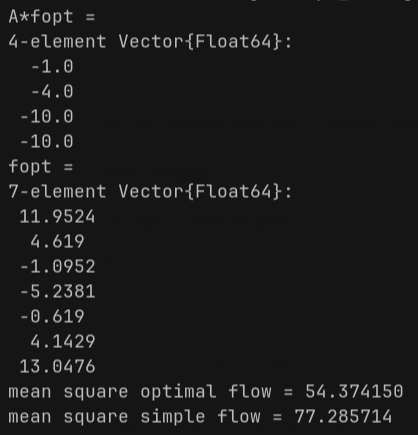
\includegraphics[width=0.4\textwidth]{img/3.png}
\end{figure}
% With
% \[
% s=
% \begin{bmatrix}
% 1\\4\\10\\10
% \end{bmatrix}
% \]
% the optimal flow is
% \[
% f^\star=
% \begin{bmatrix}
% 11.9524\\
% 4.6190\\
% -1.0952\\
% -5.2381\\
% -0.6190\\
% 4.1429\\
% 13.0476
% \end{bmatrix}
% \]
% It satisfies
% \[
% Af^\star=-s
% \]
% The mean-square flow values are
% \[
% \frac{1}{7}\|f^\star\|_2^2=54.374150
% \]
% and
% \[
% \frac{1}{7}\|f_{\mathrm{simple}}\|_2^2=77.285714
% \]
So the optimal flow has a smaller mean-square traffic level.

\subsection{Code}
\begin{lstlisting}[language={}]
using LinearAlgebra

A = [-1.0  1.0 -1.0 -1.0  0.0  0.0  0.0;
      0.0 -1.0  0.0  0.0 -1.0  0.0  0.0;
      0.0  0.0  0.0  1.0  1.0 -1.0  0.0;
      0.0  0.0  1.0  0.0  0.0  1.0 -1.0]

s = [1.0, 4.0, 10.0, 10.0]
fsimple = [5.0, 4.0, 0.0, 0.0, 0.0, 10.0, 20.0]

fopt = -A' * inv(A * A') * s
mean_square_opt = sum(fopt.^2) / length(fopt)
mean_square_simple = sum(fsimple.^2) / length(fsimple)
\end{lstlisting}
